\chapter{Introduction}
\section{Project Context}
\subsection{Sports Predictions and Machine Learning}
Sport is fundamentally a study of competition, where individuals or collectives contend to demonstrate superior skill. However, the fascination with sporting outcomes is merely a specific manifestation of a broader human impulse: the drive to reduce environmental uncertainty. This urge is not merely cultural but biological; the human brain is increasingly understood as a ``predictive processing'' organ \cite{prediction_brain}. Rather than passively awaiting sensory input, the brain acts as a proactive biological computer, constantly generating internal models to anticipate future events.

The leveraging of machine learning is an attempt to formalise and scale this innate biological capability, applying mathematical frameworks to the inherent unpredictability of competitive play. Machine learning represents a revolutionary step in human advancement, providing a newfound power to generate predictions based entirely on real, existing data, without any subconscious bias introduced. Models created by machine learning algorithms purely attempt to extract meaningful relationships between the data points provided to them, regardless of the wider context associated.

\subsection{Esports and Valorant}
Esports is a field of competitive gaming in which multiplayer titles are played by professional teams for significant prize pools. These events are broadcast to global spectators, frequently involving viewership and wagering similar to the traditional sports industry. While the mediums differ from football or cricket, the structural and commercial aspects of the industries are closely aligned.

Valorant is a prominent example of a game with a global esports community. It is a five-versus-five tactical-shooter, where each player controls a character referred to as an Agent, possessing unique abilities. Teams alternate between attacking and defending sides; the attacking objective is to plant a device known as the spike and prevent it from being defused by the defenders. Players may be eliminated during combat, remaining out of play until the following round. Consequently, rapid reaction speeds and precise hand-eye coordination are considered crucial, making Valorant a highly skilful title. Matches are won by the first team to reach 13 rounds, with sides being swapped after 12 rounds.

The Valorant Champions Tour (VCT) is an official yearly tournament hosted by the developer, Riot Games. In terms of notoriety and structure, it may be compared to the FIFA World Cup. Within this tournament, professional teams compete in a double-elimination bracket system, requiring a team to lose twice before being eliminated from the competition. A visual representation of this structure is provided in \autoref{fig:Double Elimination Graphic Example}.

\begin{figure}[h]
    \centering
    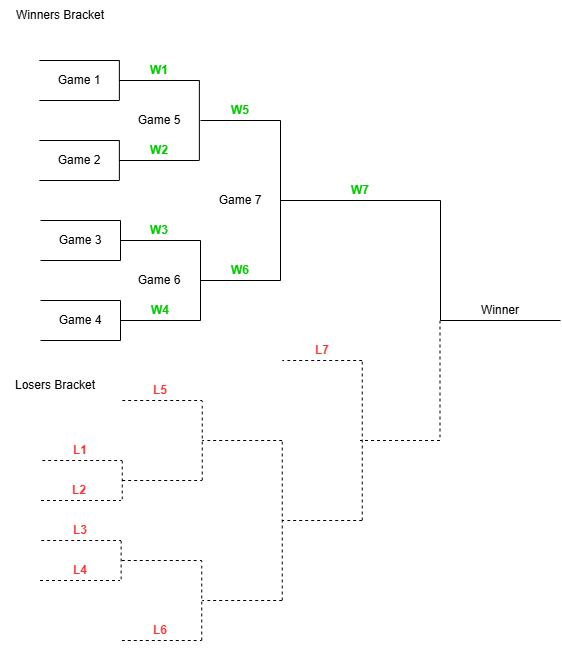
\includegraphics[width=0.7\linewidth]{./images/double-elim.png}
    \caption{An Example Flow of a Double Elimination Bracket}
    \label{fig:Double Elimination Graphic Example}
\end{figure}

The Valorant esports scene has achieved significant scale, drawing approximately two million viewers annually and awarding prize pools totalling billions of dollars over its five-year history, as documented by Esports Charts\cite{escharts_valorant}. Despite this popularity, a severe lack of sophisticated analytical tools exists for viewers seeking calculated predictions. Current online resources for VCT prediction are primarily limited to manual tracking tools for personal opinions rather than mathematically derived forecasts. Furthermore, many existing platforms are frequently littered with intrusive advertisements, detracting from the primary utility of the service and resulting in a degraded user experience.

The application of machine learning in the field of sports is already widespread, with its uses encompassing decisions such as player recruitment, performance analysis, strategy development, and notably, outcome prediction \cite{AIinSpor55:online}. These implementations have the potential to directly transfer over to the context of Valorant---informing teams on specific scenarios that they need to practise, or play styles that they are particularly vulnerable to---giving teams the opportunity to reinforce their skills before real match days.

The development of such analytical tools can be facilitated by the high degree of data fidelity inherent in digital sports. Unlike traditional athletic events, where certain metrics may be subject to human error or qualitative interpretation, data within a video game environment is fundamentally concrete; for instance, a player elimination is recorded as a definitive binary event within the game engine. Comprehensive historical datasets are maintained by third-party platforms such as VLR.gg\cite{vlr_gg}, which archive granular match statistics including win rates, round differentials, and individual player performances. The availability of this structured data provides a strong foundation for the application of machine learning models, as it allows for the extraction of precise features that are essential for accurate outcome prediction.

\section{Aims and Objectives}
The primary aim of this research project is to develop an intuitive Amazon Alexa skill capable of providing automated, data-driven predictions for VCT match outcomes. By leveraging machine learning techniques, this project seeks to address the current lack of sophisticated analytical tools available to the esports community.

To achieve this aim, the following technical and research objectives have been defined:
\label{chap:objectives}

\begin{enumerate}
\item \textbf{Data Acquisition and Pre-processing:} Source and curate a comprehensive dataset of historical VCT match results, ensuring the data is structured, normalised, and suitable for predictive modelling.
\item \textbf{Model Development:} Evaluate and implement a classification algorithm capable of outputting match outcome probabilities.
\item \textbf{Optimisation and Validation:} Perform hyperparameter tuning to maximise model accuracy and ensure generalisability on unseen data.
\item \textbf{System Integration:} Develop a pipeline for collecting data on upcoming fixtures, to ensure the model obtains current statistics.
\item \textbf{Voice User Interface (\gls{vui}) Design:} Develop an Alexa skill by defining intents and an extensive corpus of utterances, facilitating natural language interaction for match predictions.
\item \textbf{Justifiable Reasoning:} Structure the underlying data and model outputs such that the system can provide justifications for its predictions, addressing user queries such as, ``Why do you think that?''.
\item \textbf{User Evaluation and Iteration:} Conduct a formal user survey to gather qualitative and quantitative feedback on the user experience, subsequently refining the system based on these findings.
\end{enumerate}

The primary constraint identified for this project is the limited timeframe for development. Risks such as scope creep and competing academic priorities may impact the breadth of features implemented. To mitigate these risks, time-management strategies including the use of a Gantt chart and the MoSCoW (Must-have, Should-have, Could-have, Won't-have) prioritisation framework will be employed to ensure the core deliverables are met.

\section{Overview of the Report}
The remaining chapters are as follows:

\begin{itemize}
    \item \textbf{Chapter 2: Literature and Technology Survey} reviews the technology behind the project and justifies the main design choices. It compares voice assistant platforms, explains why Alexa was selected, and introduces Python and the dataset used for prediction.

    \item \textbf{Chapter 3: Requirements and Analysis} defines what the system must do and how success will be measured. It lists the key functional and non-functional requirements, then explains how the model, the Alexa skill, and the user experience will be evaluated.

    \item \textbf{Chapter 4: Planning} covers project planning and risk management. It identifies risks such as scope creep, hardware failure, and voice recognition issues, then outlines the steps used to reduce them.

    \item \textbf{Chapter 5: Design} explains the system architecture and Alexa interaction design. It describes the intents, slots, utterances, and error handling used to make the skill conversational and reliable.

    \item \textbf{Chapter 6: Implementation and Testing} describes how the system was built and tested. It covers the data preparation, feature engineering, model training, and the steps taken to deploy the final model in AWS Lambda. It also covers the manual testing employed to ensure that the skill functions as expected.

    \item \textbf{Chapter 7: Results and Discussion} presents the final results and discusses what they mean. It reports the model performance, shows example Alexa interactions, and compares the predictions with bookmaker odds. It lastly outlines any additional work that can be carried out in the future.

    \item \textbf{Chapter 8: Conclusions} concludes the report by reviewing the project outcomes against the original aims and objectives. It discusses the technologies used, and how they have proven useful, as well as summarising the next steps.
\end{itemize}